\documentclass[12pt]{amsart}
\usepackage{style}

\author{Blake Farman}
\address{Lafayette College}
\title[Exam 2 Corrections]{Exam 2 Corrections\\Math 161}
\date{October 26, 2018}

\begin{document}
\maketitle

\makenameslot

\theoremstyle{definition}
\newtheorem{thm}{}
\renewcommand{\qedsymbol}{}

\begin{thm}[15 Points]
  Find \(\dfrac{\dif{y}}{\dif{x}}\):
  \[\cos(xy)=1+\tan y\]
\end{thm}

\newpage

\begin{thm}[20 Points]
  A street light is mounted at the top of a 15-ft-tall pole.
  A person 6 ft tall walks away from the pole with a speed of 5 ft/s along a straight path.
  How fast is the tip of the person's shadow moving when the person is 40 ft from the pole?\\
  (Hint: The length of the shadow is measured from the person to the tip of the shadow; the rate at which the tip of the shadow is moving is measured from the pole to the tip of the shadow.)
\end{thm}

\vspace{3in}

\begin{thm}[15 Points]
  Find the value or values of $c$ that satisfy the conclusion of the Mean Value Theorem for the function $f(x)=x^3 - 2x^2 -4x + 2$ on $[-2,2]$.
\end{thm}

\newpage

\begin{thm}[15 Points]
  Find the absolute maximum and minimum values of $f(x)=2x^3 - 3x^2 -12x + 1$ on $[-2,3]$.
\end{thm}

\vspace{2in}
\begin{thm}[20 Points]
  Sketch the curve $$f(x)=\frac{x^2}{x-1}$$
  \begin{enumerate}[(a)]
  \item\label{sketching first step}
    State the domain of \(f\).
    \vspace{1in}
    
  \item
    Find the intercepts for \(f\) and express them as an \((x,y)\) pair.
    Write NONE if there are none.\\ \\
    x-intercept(s):\hskip .5 truein \hrulefill\\ \\
    y-intercept:\hskip .5 truein \hrulefill
  \item
    Is \(f\) even, odd, or neither?
    What type of symmetry does \(f\) have?
    \vspace{1in}
  \item
    Find the asymptotes of \(f\).
    Write NONE if there are none.\\ \\
    Horizontal:\hskip .5 truein \hrulefill\\ \\
    Oblique:\hskip .5 truein \hrulefill\\\ \\
    Vertical:\hskip .5 truein \hrulefill
    \newpage
  \item
    Find the intervals where \(f\) is increasing and decreasing.
    Write NONE if not applicable.\\ \\
    Increasing:\hskip .5 truein \hrulefill\\ \\
    Decreasing:\hskip .5 truein \hrulefill
    \vspace{3in}
  \item
    State the local extrema as an \((x,y)\) pair.
    Write NONE if not applicable.\\ \\
    Local maximum value(s):\hskip .5 truein \hrulefill\\ \\
    Local minimum value(s):\hskip .5 truein \hrulefill
  \item\label{sketching penultimate step}
    Find the intervals on which \(f\) is concave up and concave down.
    State the inflection points.
    Write NONE if not applicable.\\ \\
    Concave Up:\hskip .5 truein \hrulefill\\ \\
    Concave Down:\hskip .5 truein \hrulefill\\ \\
    Inflection Points:\hskip .5 truein \hrulefill
    \vspace{2in}
  \item
    Use your answers to Parts~\eqref{sketching first step}-\eqref{sketching penultimate step} to sketch the graph of \(f\).
    Be sure that your graph is labeled and neat.
    Messy/incoherent graphs will receive zero points.
    \begin{center}
      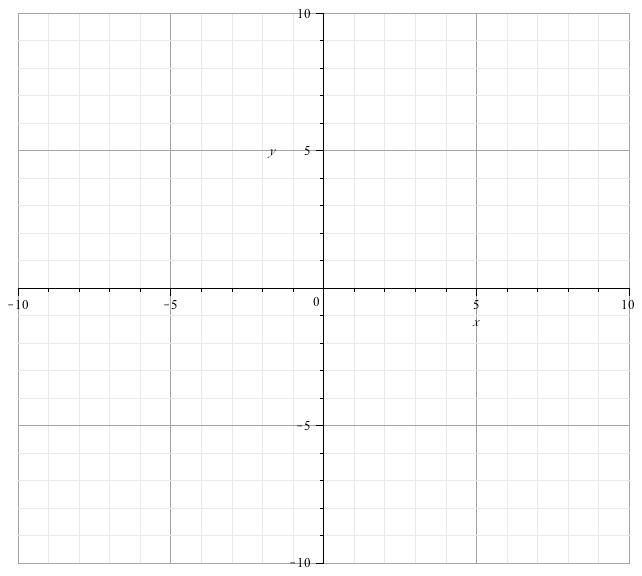
\includegraphics[scale=0.5]{graphpaper.jpg}
    \end{center}
  \end{enumerate}
\end{thm}
\end{document}
